%!TEX root = thesis.tex
\chapter{Phonon Coupling in Semiconductor Bi-layers and Tri-layers}
\label{chap:layered}
%INTRODUCTION%
\section{Introduction} \blfootnote{Portions of this chapter have originally been published in \cite{ownCoupling1} ``Enhancing Thermal Transport in Layered Nanomaterials" (2018), \textit{Scientific Reports}, Vol. 8 (1880); in \cite{ownCoupling2} ``Modulating Thermal Conduction via Phonon Spectral Coupling" (2018), \textit{Journal of Applied Physics}, Vol. 124 (124302); and in \cite{ownKK1} ``Unconventional Thermal Transport in Thin Film-on-Substrate Systems" (2018), \textit{Journal of Physics D: Applied Physics}, Vol. 51 (365302). Reproduced from \cite{ownCoupling1} under a CC BY 4.0 License, from \cite{ownCoupling2} with permission from AIP Publishing, and from \cite{ownKK1} with permission from IOP Publishing.}
The ability to reduce heat conduction at nanoscale has been propelled by advances in the understanding of phonon transport processes in semiconductors. In recent years, suppression of thermal conduction by orders of magnitude has been achieved through the diffuse scattering of phonons at nanostructure surfaces. Nanowires, thin-films, nanotubes, superlattices, polycrystals, and nanocomposites with extremely low thermal conductivities have been introduced which find applications as efficient thermoelectric materials \cite{RN136,NW_hochbaum,RN417,RN29,RN88,RN158,RN320,RN132,RN394,RN393,RN240,RN294,ownNW,ownTF,ownSpatialTF}. Nanostructuring has thus primarily been used to reduce the thermal conductivities for a wide range of temperatures, and was the underlying motivation of \Cref{chap:predictive,chap:diff_boundary,chap:nt}. 
\par However, under a rational material design paradigm to create thermal materials, it is paramount to possess the ability to achieve both very low and very high thermal conductivities. Accessing the ability to enhance thermal conduction at nanoscale requires the development of novel approaches based on a deep understanding of phonon transport behavior. Furthermore, progress in many technological areas is hinged upon enhancing thermal transport. For instance, the performance of micro- and nano-electronic devices is hindered by the creation of hot-spots and high working temperatures as small sizes limit efficient heat dissipation (see \Cref{chap:intro}). This need to obtain increased thermal conductivities has also motivated recent efforts to study the effects of interfacial disorder \cite{RN265}, extremely low temperature \cite{RN397}, and texturing of interfaces \cite{RN398} on changes in thermal conductance. Additionally, being able to devise physical mechanisms that would allow to increase thermal conduction is of crucial importance in the efficiency of electronic and optoelectronic devices. For example, long laser lifetimes necessitate an upper bound on the temperature of active layers thus making efficient heat removal a crucial aspect of designing laser systems \cite{ownKK1}. In addition, heat accumulation in the depletion layer of photo-detectors can lead to device failure at high optical power \cite{kk-li2003}. An increase in dark current with temperature leading to increased power dissipation can also result in thermal runaway and failure \cite{kk-Lorenzen2001}. In contrast to the extensive amount of work on achieving reduced thermal conduction in nano systems, approaches that can enhance thermal conduction have been limited. In particular, increased thermal dissipation in thin-films and layered nanomaterials would have a critical impact on performances of electronic and optoelectronic devices.
\par In this chapter, we formulate a mathematical model to study thermal transport in layered nanomaterials based on solving the BTE for non-equilibrium phonon populations. We briefly discussed such method in \Cref{chap:diff_boundary} for free-standing thin-films. Here, we show a more generic development that can account for both backward scattering (i.e., reflection) and forward scattering (i.e., transmission) of phonons at an interface between two nanostructured semiconductors. Using this model, we elucidate the role of phonon coupling on the local thermal conductivity of each layer in the structure. Specifically, we show the impact of phonon coupling on thermal conductivity of Si and Ge layers in a Si-Ge-Si tri-layer structure and highlight that phonon coupling can be used to enhance the thermal conductivity of the Ge layer. We analyze the root-cause of such an occurrence with our model and study the role of different structural parameters, including surface properties and layer sizes. Finally, we apply the model to technologically important structures, i.e. film-on-substrate architectures (FOS), and show that thermal conduction in these film-on-substrate systems is distinct from free-standing thin films highlighting the role of phonon coupling for design of devices and in interpreting read-out from experiments.
%METHOD
\section{Method}
%Figure
\begin{figure}[hbt]
  \centering 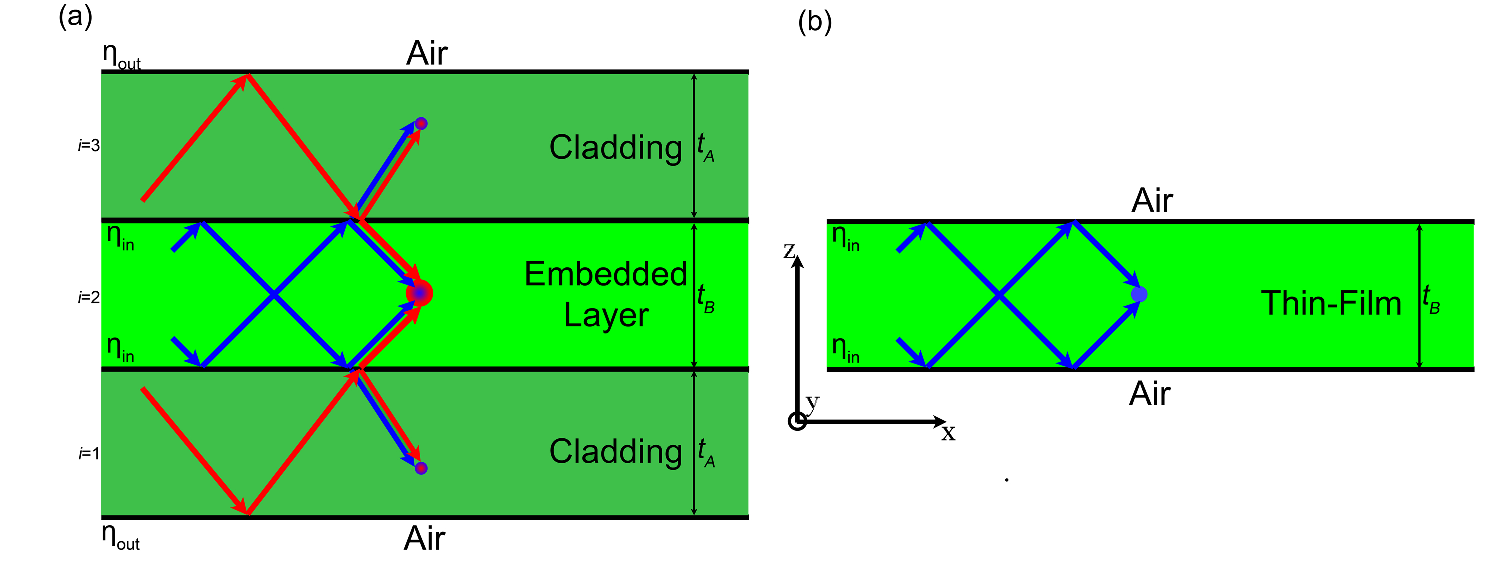
\includegraphics[width=1.0\textwidth,scale=1.5]{ch5/Fig1.pdf}
  \caption{(a) A tri-layer architecture (A-B-A) made of an embedded B layer with thickness $t_2$ and cladding A layers with thicknesses $t_1$. The roughness of the inner surface between embedded and cladding layers is $\eta_{in}$ and the roughness of the cladding-air outer interface is $\eta_{out}$. Arrows illustrate the phonon injection mechanism, wherein phonons from the cladding layers A couple across the inner interface to net replace phonons in the embedded layer B. As a result of phonon coupling, the thermal conductivity $\kappa_{\text{B}}$ of the embedded layer can be enhanced or reduced from the free-standing thin-film value $\kappa_{\text{B-free}}$ as shown in (b). Note that the arrow colors are illustrative, and phonons in each layer have the dispersion and relaxation rates of the corresponding layer material (i.e., after coupling, phonons do not keep the properties of the layer in which they originated).}
    \label{fig:ch5_schematic_coupling}
\end{figure}
We first analyze tri-layer systems comprising an inner embedded layer of material B, which is cladded on both the sides by layers of material A with same thickness [\Cref{fig:ch5_schematic_coupling}] to create A-B-A layered architectures. The inner interface between embedded and cladding layers and the outer interface between cladding layers and air have different surface properties. Thus, the tunable structural properties that determine phonon transport are the thicknesses of the layers and the inner and outer surface properties. To study the fundamental phonon transport processes occurring in these structures, we use the Boltzmann transport equation, which allows to accurately incorporate detailed surface characteristics in thermal conductivity numerical predictions. The general solution of phononic population \gls{f}$_i$ can be obtained in terms of the deviation in phononic population \gls{g}$_i$ from the equilibrium distribution \gls{f}$_i^{BE}$ in layer $i$, at a distance $z$ from the interface upon application of a gradient ${\partial T}/{\partial x}$ in the in-plane $x$ direction to the entire tri-layer structure, and is given by \cite{RN396,ownSpatialTF,book_Ziman}\footnote{also see \Cref{eq:ch3-5}},
\begin{equation}
  g_i^\pm=  -v_{i|x} \tau_{i}\frac{\partial T}{\partial x}\frac{\partial f_{i}^{BE}}{\partial T}\Bigg(1+\Phi_{i}^\pm\exp\Big(\dfrac{\mp z}{\tau_{i} |v_{i}\cos \theta_i|}\Big) \Bigg)
\label{eq:ch5-gpm}
\end{equation}
where $v_{i|x}$ denotes the x-component of the phonon group velocity $\vec{v}$, \gls{tau} is the relaxation time, \gls{thetai} is the angle of incidence at the interface, and $\Phi_i^\pm$ are determined by requiring the phonon distribution function to satisfy the boundary conditions described below. We note that $g^\pm$ depends on the direction of phonon propagation indicated by + and - symbols for positive and negative z-components of the wave-vector, respectively. The boundary conditions for the tri-layer system at the outer cladding-air interfaces are,
\begin{equation}
  g_1^+= p_{out}\, g_1^- \: \textrm{at}  \: z=0  
\end{equation}
and, 
\begin{equation}
  g_3^-= p_{out}\, g_3^+ \: \textrm{at} \: z=t_1+t_2+t_1
\end{equation}
where $p_{out}$ is the specularity of the cladding air interface and $t_2$ is the thickness of the embedded layer (i = 2), which is cladded between two layers of $t_1$ thickness each ($i$ = 1 and 3). We note that $p_{out}$ is a function of both surface and incident phonon properties and can be determined using BK approach (see \Cref{sec:BK}). At the inner interface between cladding and embedded layer, in addition to a fraction of incident phonons get specularly reflected ($P_{ij}$), a fraction of phonons can also get specularly transmitted ($T_{ij}$), while the rest are diffusively scattered. An extension of the BK scattering theory is required to account for the transmission effects and is detailed in Refs. \cite{RN396,RN340}. Under such an approach the specularly reflected and transmitted phonon fractions can be obtained by, 
\begin{equation}
P_{ij} = Z_{ij}^{2} \exp{(-4\eta^{2} k_{i}^{2} \cos^{2} \theta_{i})}
\label{eq:bezak_reflection}
\end{equation} 
and
\begin{equation}
T_{ij} = (1-Z_{ij}^{2}) \exp{(-\eta^{2} (k_{i} \cos\theta_{i}-k_{j}\cos\theta_{j})^{2})}
\label{eq:bezak_transmission}
\end{equation} 
respectively. In these expressions, $k_i$ and $k_j$ are the incident and transmitted phonon wavenumbers, \gls{thetai} and \gls{thetai} are the incidence and transmission angles, and $Z_{ij}$ is the acoustic impedance between the two media across the surface dependent on the densities $\rho$ and phonon velocities $v$ in the two media.
\begin{equation}
Z_{ij} = \Bigg( \frac{ \rho_{i}v_{i}\cos\theta_{i}-\rho_{j}v_{j}\cos\theta_{j} }{ \rho_{i}v_{i}\cos\theta_{i}+\rho_{j}v_{j}\cos\theta_{j} } \Bigg)^{2}
\label{eq:bezak_acc_mismatch}
\end{equation} 
The role of surface conditions can be explicitly observed, and it is expected that the probability of specular reflection and transmission of phonons diminishes with increasing surface disorder. Note that since the momentum component parallel to the surface is preserved for specularly scattered phonons, it gives rise to the preservation of reflection angle and Snell’s law for specular transmission.
\begin{equation}
k_{i}\cos\theta_{i} = k_{j}\cos\theta_{j}
\label{eq:snells_law}
\end{equation} 
Additionally, the effects of correlations between surface asperities are quantified using the correlation length \gls{cl} which impacts the coefficients $P_{ij}$ and $T_{ij}$ and is accounted via surface shadowing as discussed in \Cref{sec:BK}. If a particular mode is subject to total internal reflection or there is no overlap between phonon dispersions, the phonon transmission is $T_{ij} = 0$ and there is no phonon spectral coupling. For these modes, surface scattering and mean-free-path reduction are equivalent to those in a free-standing thin-film. By considering phonon reflection and transmission, the boundary conditions at the internal surfaces are,
\begin{equation}\label{BM2}
\begin{aligned}
 g_1^- &= P_{12}g_1^+ + T_{12}g_2^- && \text{at}\; z=t_1\\
 g_2^+ &= P_{21}g_2^- + T_{12}g_1^+ && \text{at}\; z=t_1\\
 g_2^- &= P_{23}g_2^+ + T_{23}g_3^- && \text{at}\; z=t_1+t_2\\
 g_3^+ &= P_{32}g_3^- + T_{23}g_2^+ && \text{at}\; z=t_1+t_2
\end{aligned}
\end{equation}
Thus, numerical solutions of non-equilibrium phononic populations are obtained by evaluating these equations using LAPACK solvers in FORTRAN. The thermal properties of individual layer $i$ are then evaluated using \Cref{eq:phonon_fourier}. Thus, using a mode-by-mode numerical methodology based on the Boltzmann transport equation, we are able to include phonon coupling at the interfaces in the computation of thermal transport properties in tri-layer architectures. Moreover, the methodology described above can further be extended to layered nanomaterials with arbitrary number of layers by modifying the appropriate boundary conditions to evaluate the deviation functions for each layer, as will be done in \Cref{chap:slxp}.
\section{Results and Discussion}
In order to analyze the development of thermal conductivity, we focus on a Si-Ge-Si architecture. The mutual interaction between phonons of two layers is based on the ability of phonons to be transmitted at the interface. In general, upon interacting with a surface, a fraction of phonons undergoes specular reflection and transmission, while the rest are randomized along all angular directions. First, we leverage this mutual exchange of phonons via transmission, to increase the thermal conductivity of a germanium thin-film embedded between silicon layers with respect to a free-standing germanium thin-film with the same physical properties. Second, we show the origins of this increase of Ge layer conductivity comes at the cost of the conductivity of the Si layer.  
%Figure
\begin{figure}[hbt]
  \centering 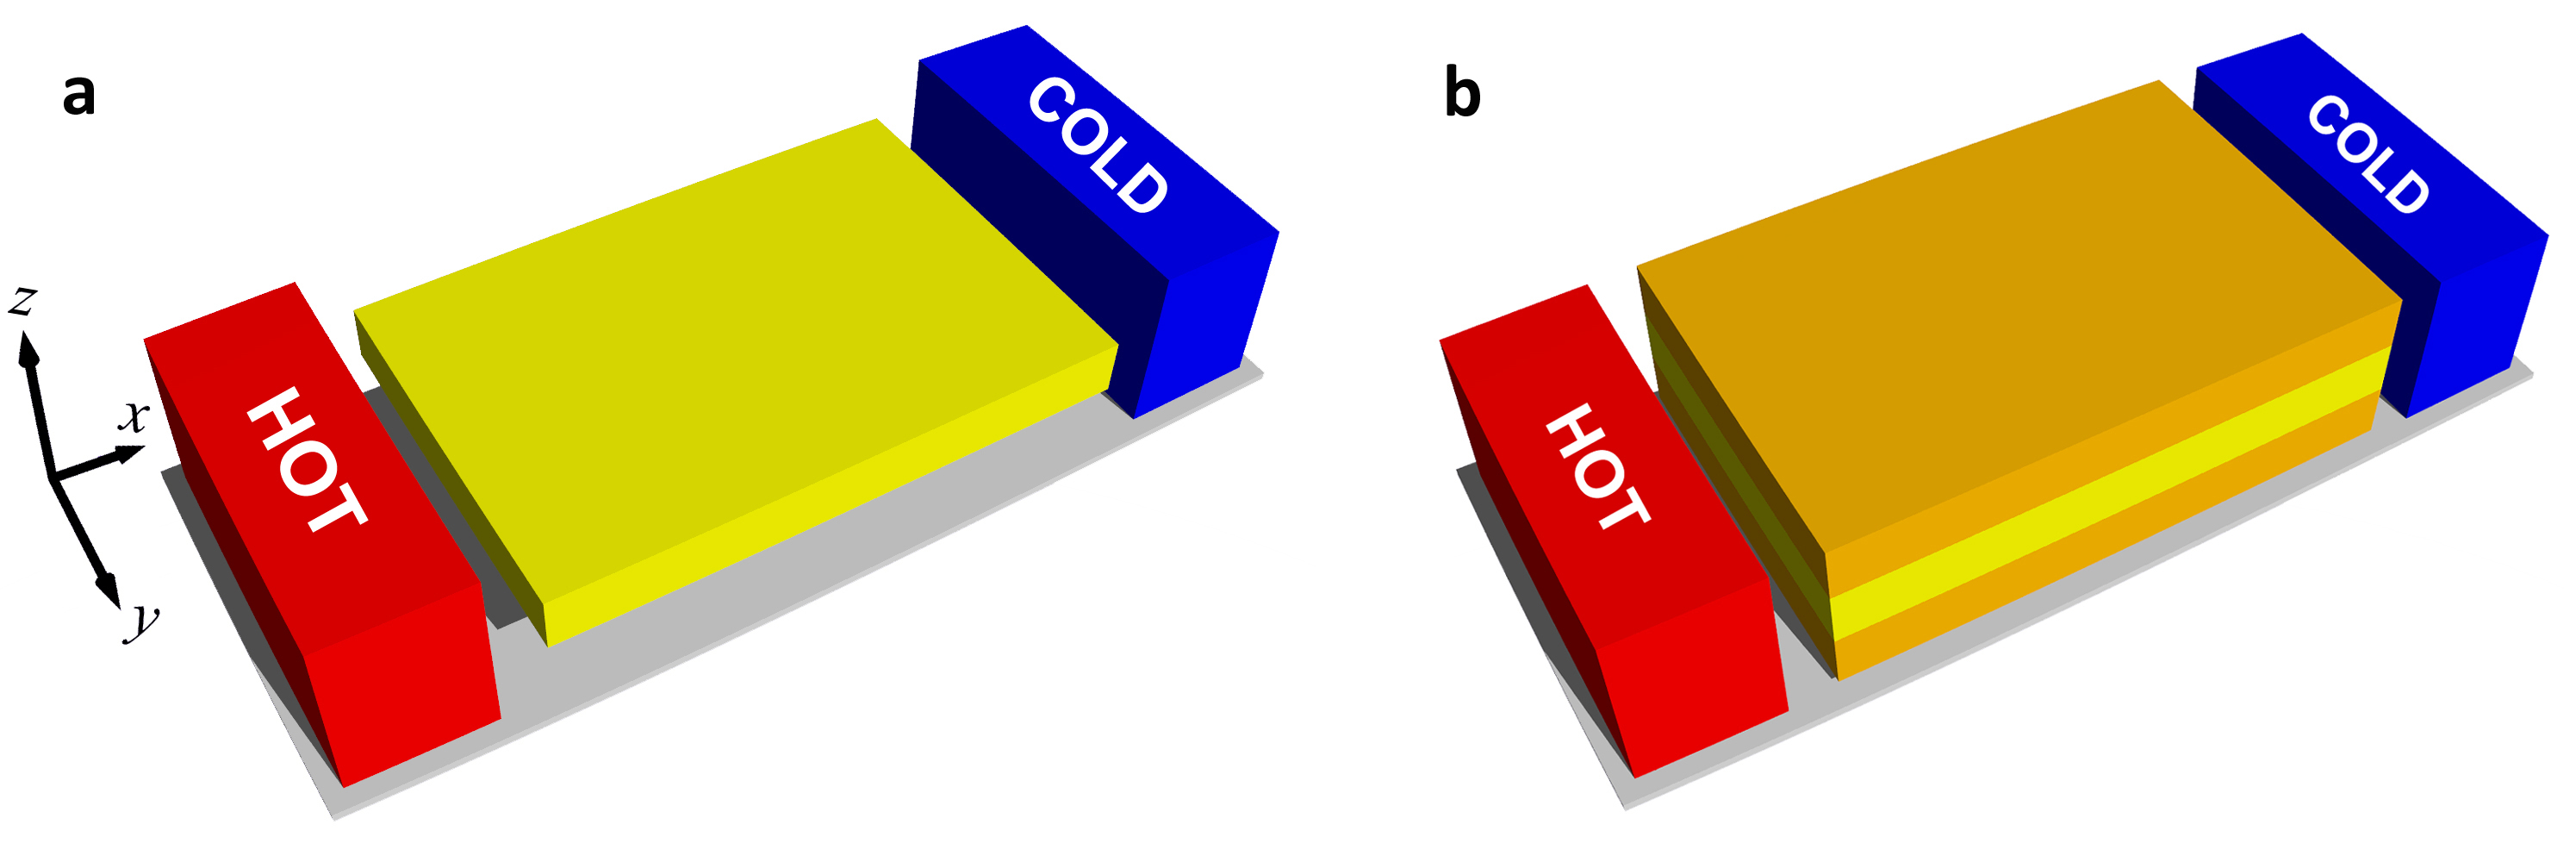
\includegraphics[width=1.0\textwidth]{figures/ch5/Fig1tl.jpg}
  \caption{Tri-layer superlattice nanostructure in (a). Schematic for a free-standing germanium thin film (yellow) in (b). By embedding the germanium thin film between silicon layers (orange) the thermal conductivity of the germanium film can be increased. The temperature gradient is applied to the whole structure in the $x$-direction.}
  \label{fig:ch5-tl}
\end{figure}

\subsection{Enhancement of Ge Layer Conductivity}
The calculated thermal conductivities of a germanium thin film in the tri-layer structure are shown in \Cref{fig:ch5-enh1} as a function of the thickness of the silicon cladding layer $t_{\text{Si}}$, where a significant enhancement in thermal conductivity of the germanium film over the free-standing counterpart is observed. Note that the dispersion relations in the [100] direction were used for these calculations, as reported in literature \cite{RN388}. We find that it is possible to nearly double the thermal conductivity (\textgreater90\% enhancement) of a 10 nm germanium thin-film by using two 1 \si{\micro}m thick silicon samples as cladding. Two cases for the specularities of the cladding-air interface are considered, \gls{p}$_{out}$ = 0 and 1, to cover all possibilities in terms of the quality of the silicon-air interfaces \cite{book_Ziman}. The germanium-silicon interface has roughness \gls{eta} = 0.1 nm. A germanium thin-film with given physical properties (surface roughness, correlation length, and thickness) without any cladding is used as the baseline measure for comparison. It is also observed that the larger the cladding thickness, the larger the increase in the thermal conductivity of the germanium thin film. This is because, for larger thicknesses of the silicon cladding layers, phonon scattering at the interfaces is reduced (see \Cref{chap:predictive}) and silicon phonon mean free paths are not shortened previously to their injection in germanium. Note that the enhancement of conductivity via injection of phonons is not unbounded with increasing cladding thickness, rather it begins to saturate as shown in \Cref{fig:ch5-enh1}(a). Clearly, increasing cladding thickness beyond the saturation limit is of no additional advantage from the perspective of enhancement, as the thermal conductivity contribution of phonons that can interact with the embedded layer has already been maximized. The specularity of the cladding-air interface is another factor that can influence the injection of phonons into the embedded layer. At the same cladding thickness, the observed enhancement of thermal conductivity in the embedded layer is higher for larger cladding-air surface specularities. This behavior is consistent since a more diffuse cladding shortens the phonon mean-free-paths, and therefore a larger thickness is required to improve the injection efficiency. Note that at sufficiently large cladding thicknesses, the impact of the quality of the silicon-air interface on germanium thermal conductivity enhancement begins to diminish and in the case of a bulk silicon cladding it would be expected that the enhancement is the same irrespective of the roughness of the cladding-air surface. Note that coherent modifications to the phonon dispersion relations can be neglected at room temperature owing to the choice of embedded layer thicknesses \cite{RN372}.
%Figure
\begin{figure}[hbtp]
  \centering 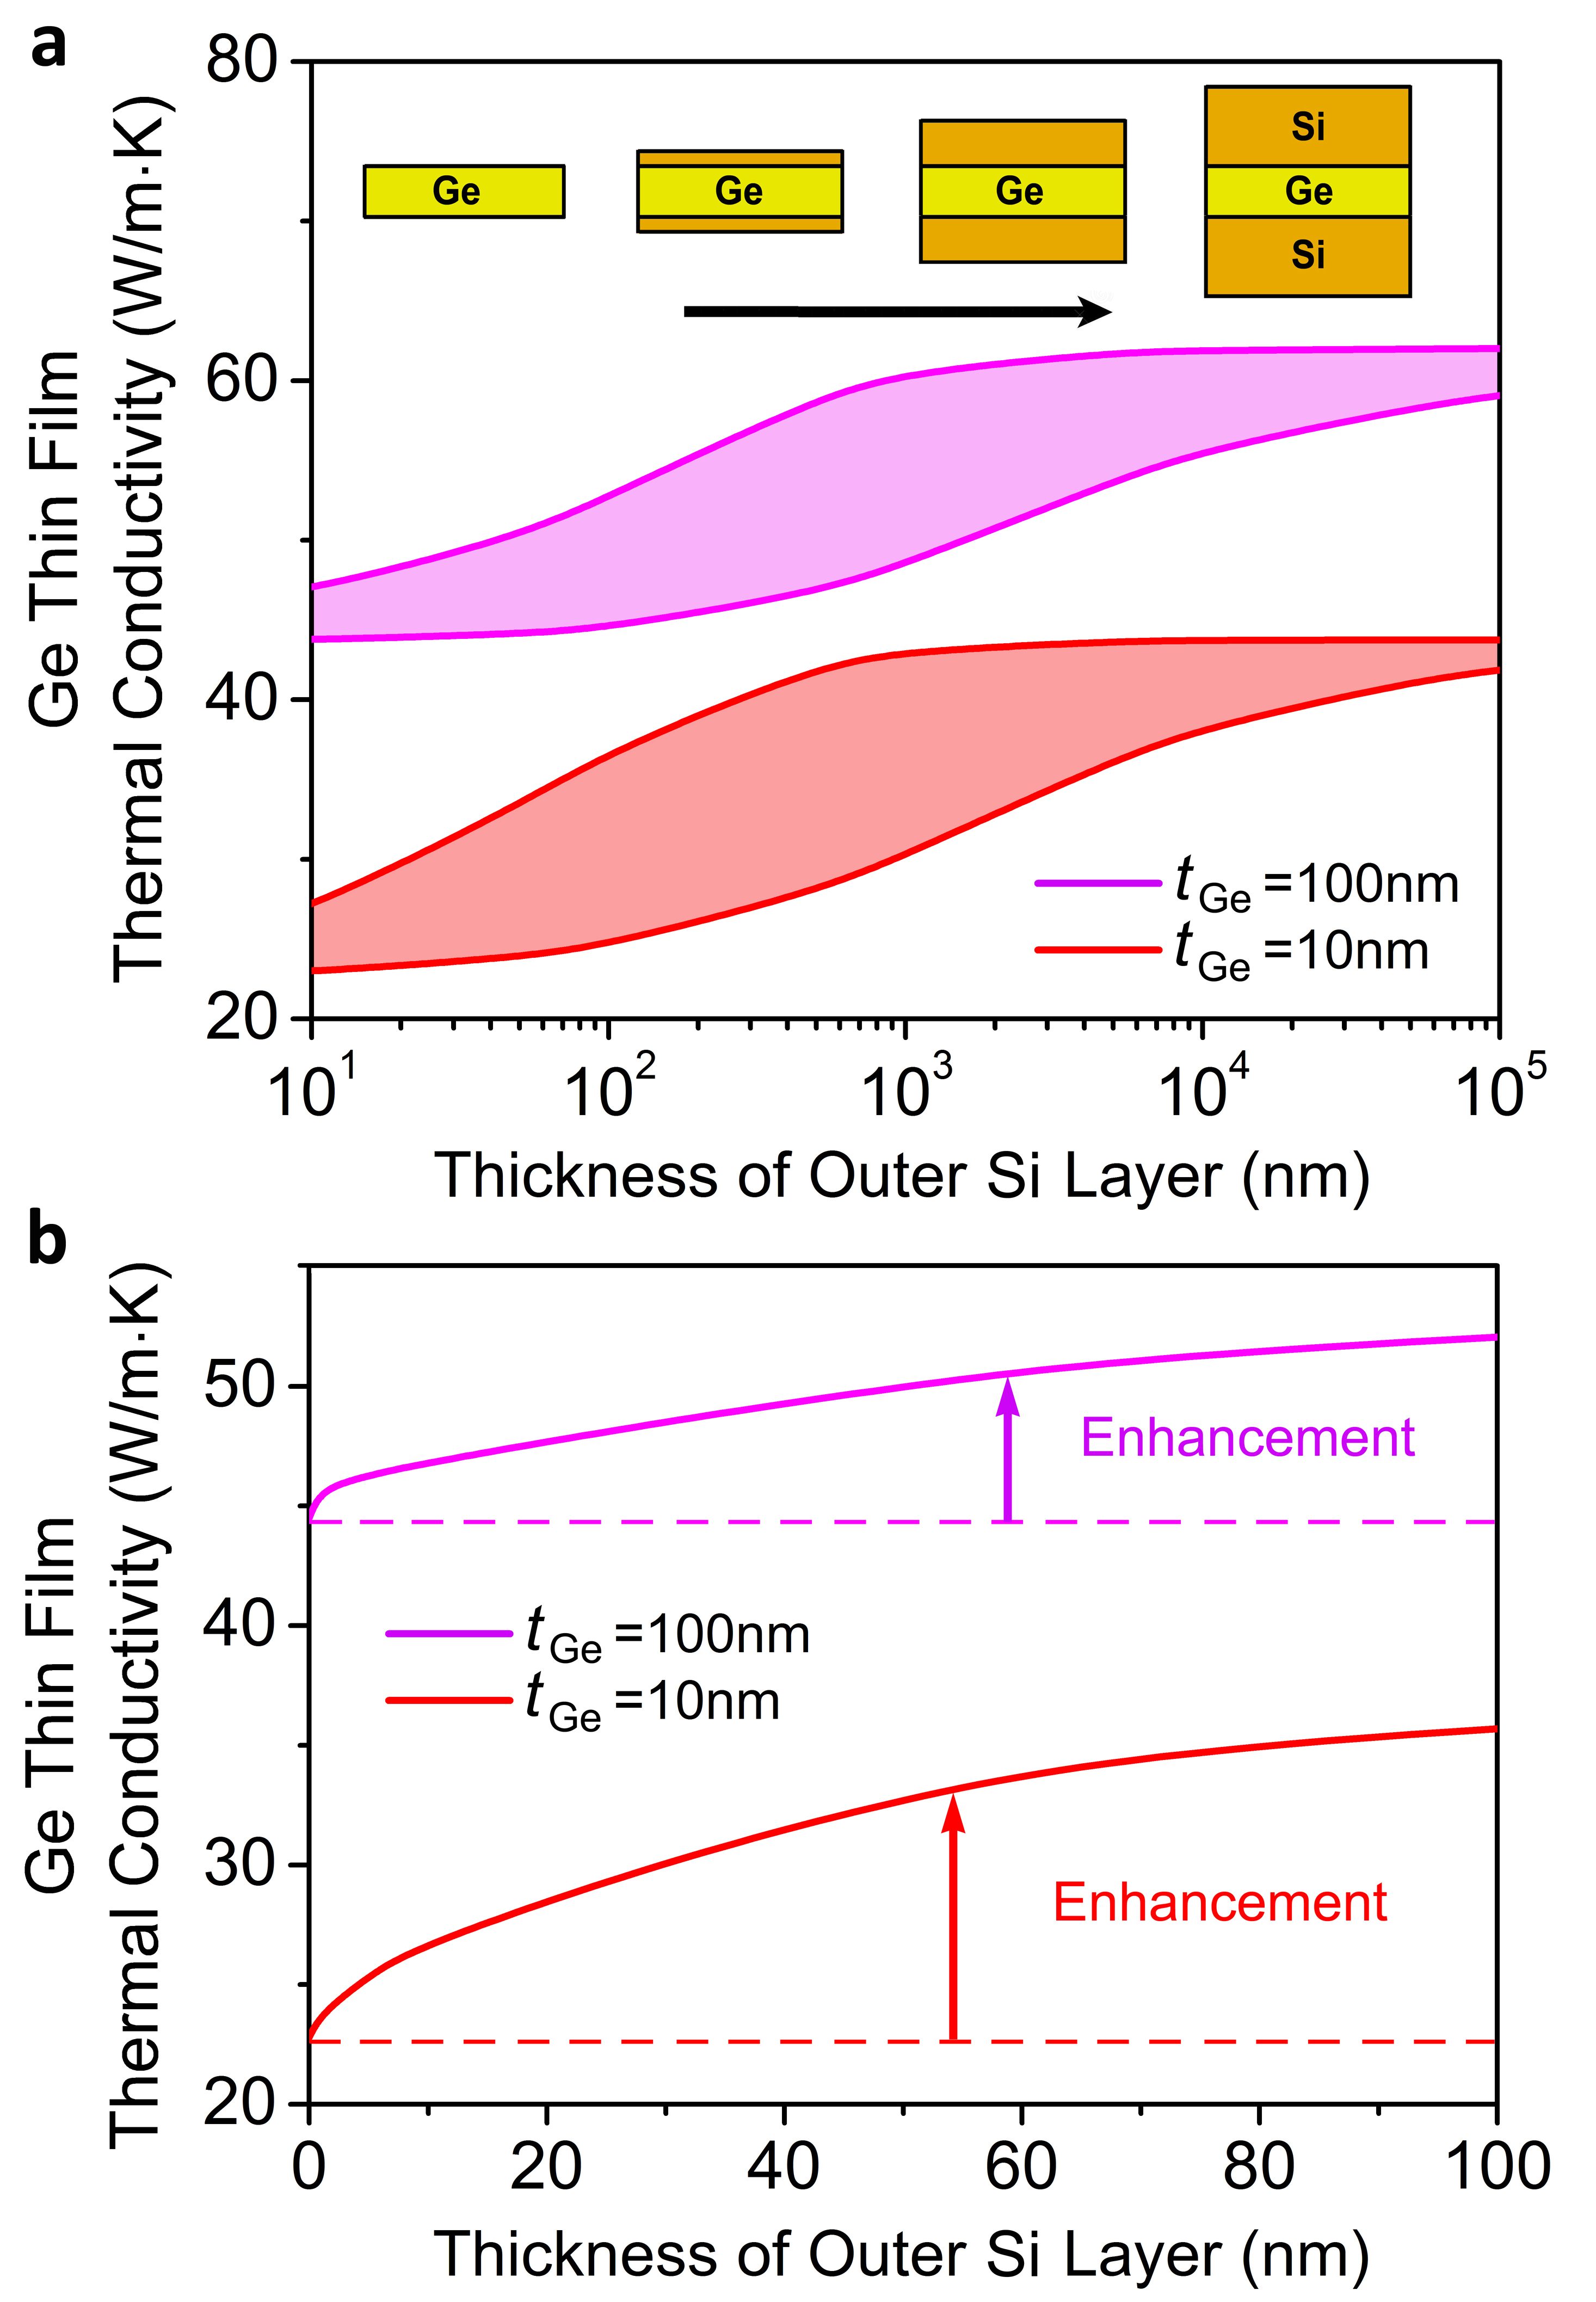
\includegraphics[width=0.80\textwidth]{figures/ch5/Fig1-enh.jpg}
  \caption{Increased thermal conductivity. (a) Colored areas show the enhancement in the thermal conductivity of a germanium thin film as a function of increasing thickness of the silicon cladding layer. The top and bottom lines correspond to silicon-air surface specularities \gls{p} = 1 and \gls{p} = 0, respectively, covering all possibilities in terms of surface roughness. The germanium-silicon interface has roughness \gls{eta} = 0.1 nm and correlation length \gls{cl} = 20\gls{eta}. (b) Enhanced thermal conductivity of an embedded germanium film (solid lines) with respect to a free-standing germanium thin film (dotted lines) having the same physical properties. The germanium-silicon interface has \gls{eta} = 0.1 nm, \gls{cl} = 20\gls{eta} while the silicon-air surface specularity is equal to one. The temperature gradient is in the plane of the films.}
    \label{fig:ch5-enh1}
\end{figure}
\par \Cref{fig:ch5-enh2} show the impact of silicon-germanium interface roughness on the increased thermal conductivity of the germanium film. Significant enhancements ($\sim$100\%) in thermal conductivities of the 10 nm embedded layer with roughness values in range of \gls{eta} = 0.1–0.4 nm can be achieved by using 1 \si{\micro}m silicon layers as cladding. Additionally, with increasing thickness of the embedded germanium layer, the maximum enhancement is reduced as the cladding is only able to inject phonons into a part of the thicker embedded germanium film. That is, the proportion of region in the germanium layer that is able to augment its local conductivity with the injected phonons from silicon decreases, leading to a smaller enhancement in thermal conductivity. Another interesting observation is that the thermal conductivity of a germanium thin-film can be enhanced beyond the bulk thermal conductivity of germanium at room temperature (60 W/m-K) using the described tri-layer architecture. However, it is important to note that the thermal conductivity enhancement in the embedded-layer occurs at the cost of reducing the thermal conductivity of the silicon cladding layer (as compared to a baseline silicon film of similar physical properties). In general, the reduction in thermal conductivity of the cladding layer would depend on structural properties including layer thicknesses and roughness. For a large ratio of cladding-to-embedded layer thickness, this reduction would be small since phonons from a small region near the interface would be able to couple across the interface. In simple words, the cladding layers allow for an enhancement of the thermal conductivity in the embedded layer by injecting phonons with sufficiently long mean-free-paths across the interface. 
%Figure
\begin{figure}[hbt]
  \centering 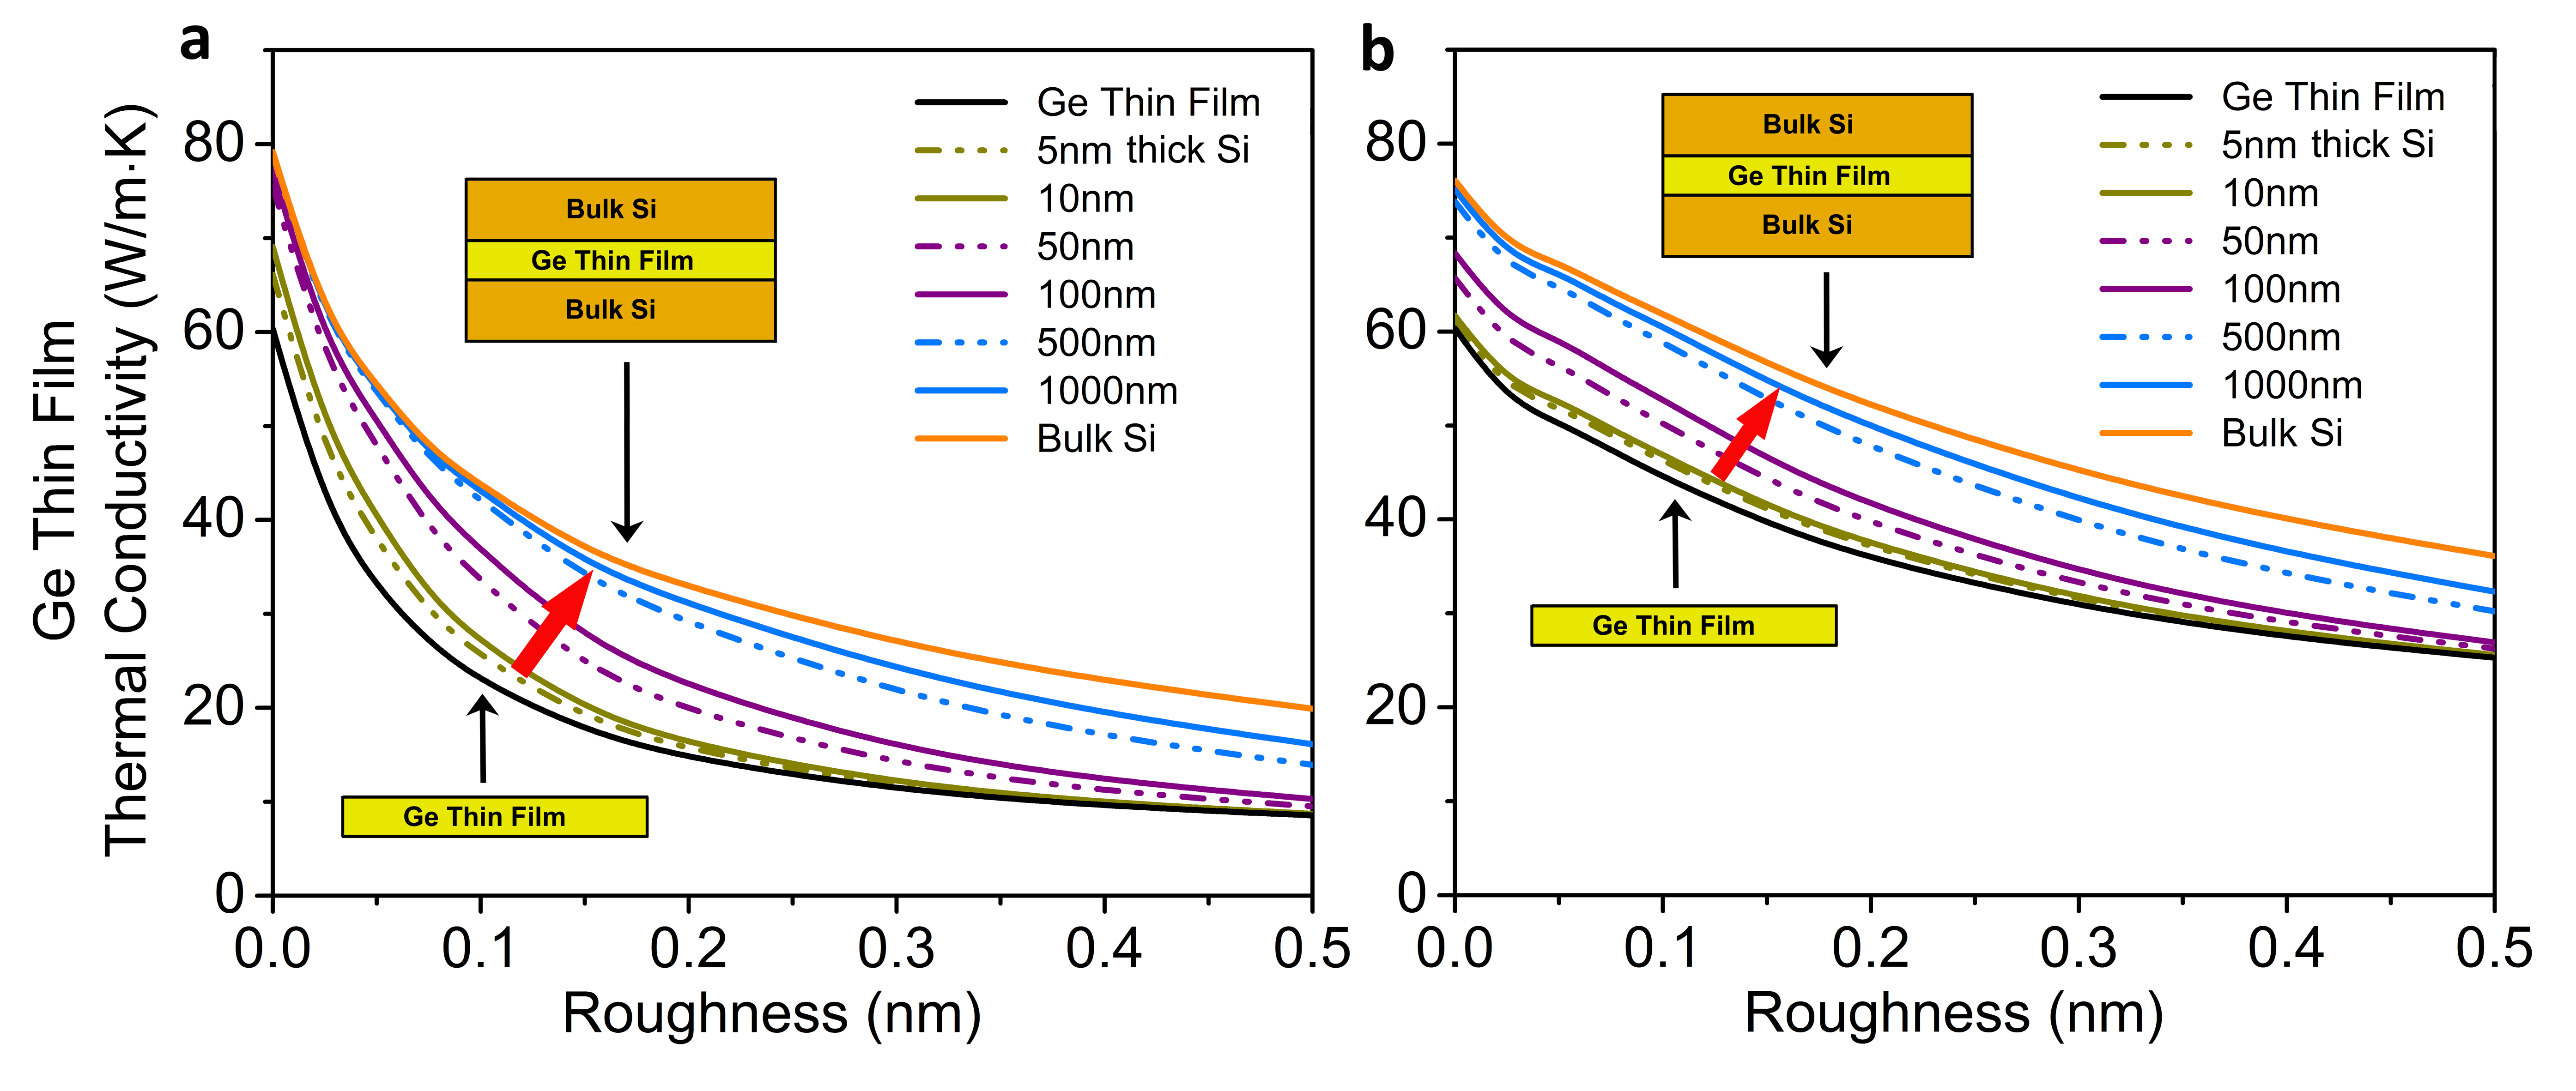
\includegraphics[width=1.0\textwidth]{figures/ch5/Fig2-enh.jpg}
  \caption{Enhanced heat conduction. Thermal conductivity increase for the embedded germanium film as a function of the silicon-germanium interface roughness. The germanium thin film thickness is (a) $t_{\text{Ge}}$ = 10 nm and (b) $t_{\text{Ge}}$ = 100 nm. Color lines correspond to different thicknesses of the silicon layers, increasing from no silicon layer to bulk silicon (indicated by red arrow). The enhancement in the thermal conductivity of the embedded germanium film, with respect to the free-standing germanium thin film with same properties, is observed for various surface roughnesses and silicon layer thicknesses.}
  \label{fig:ch5-enh2}
\end{figure}
%Figure
\begin{figure}[hbt]
  \centering 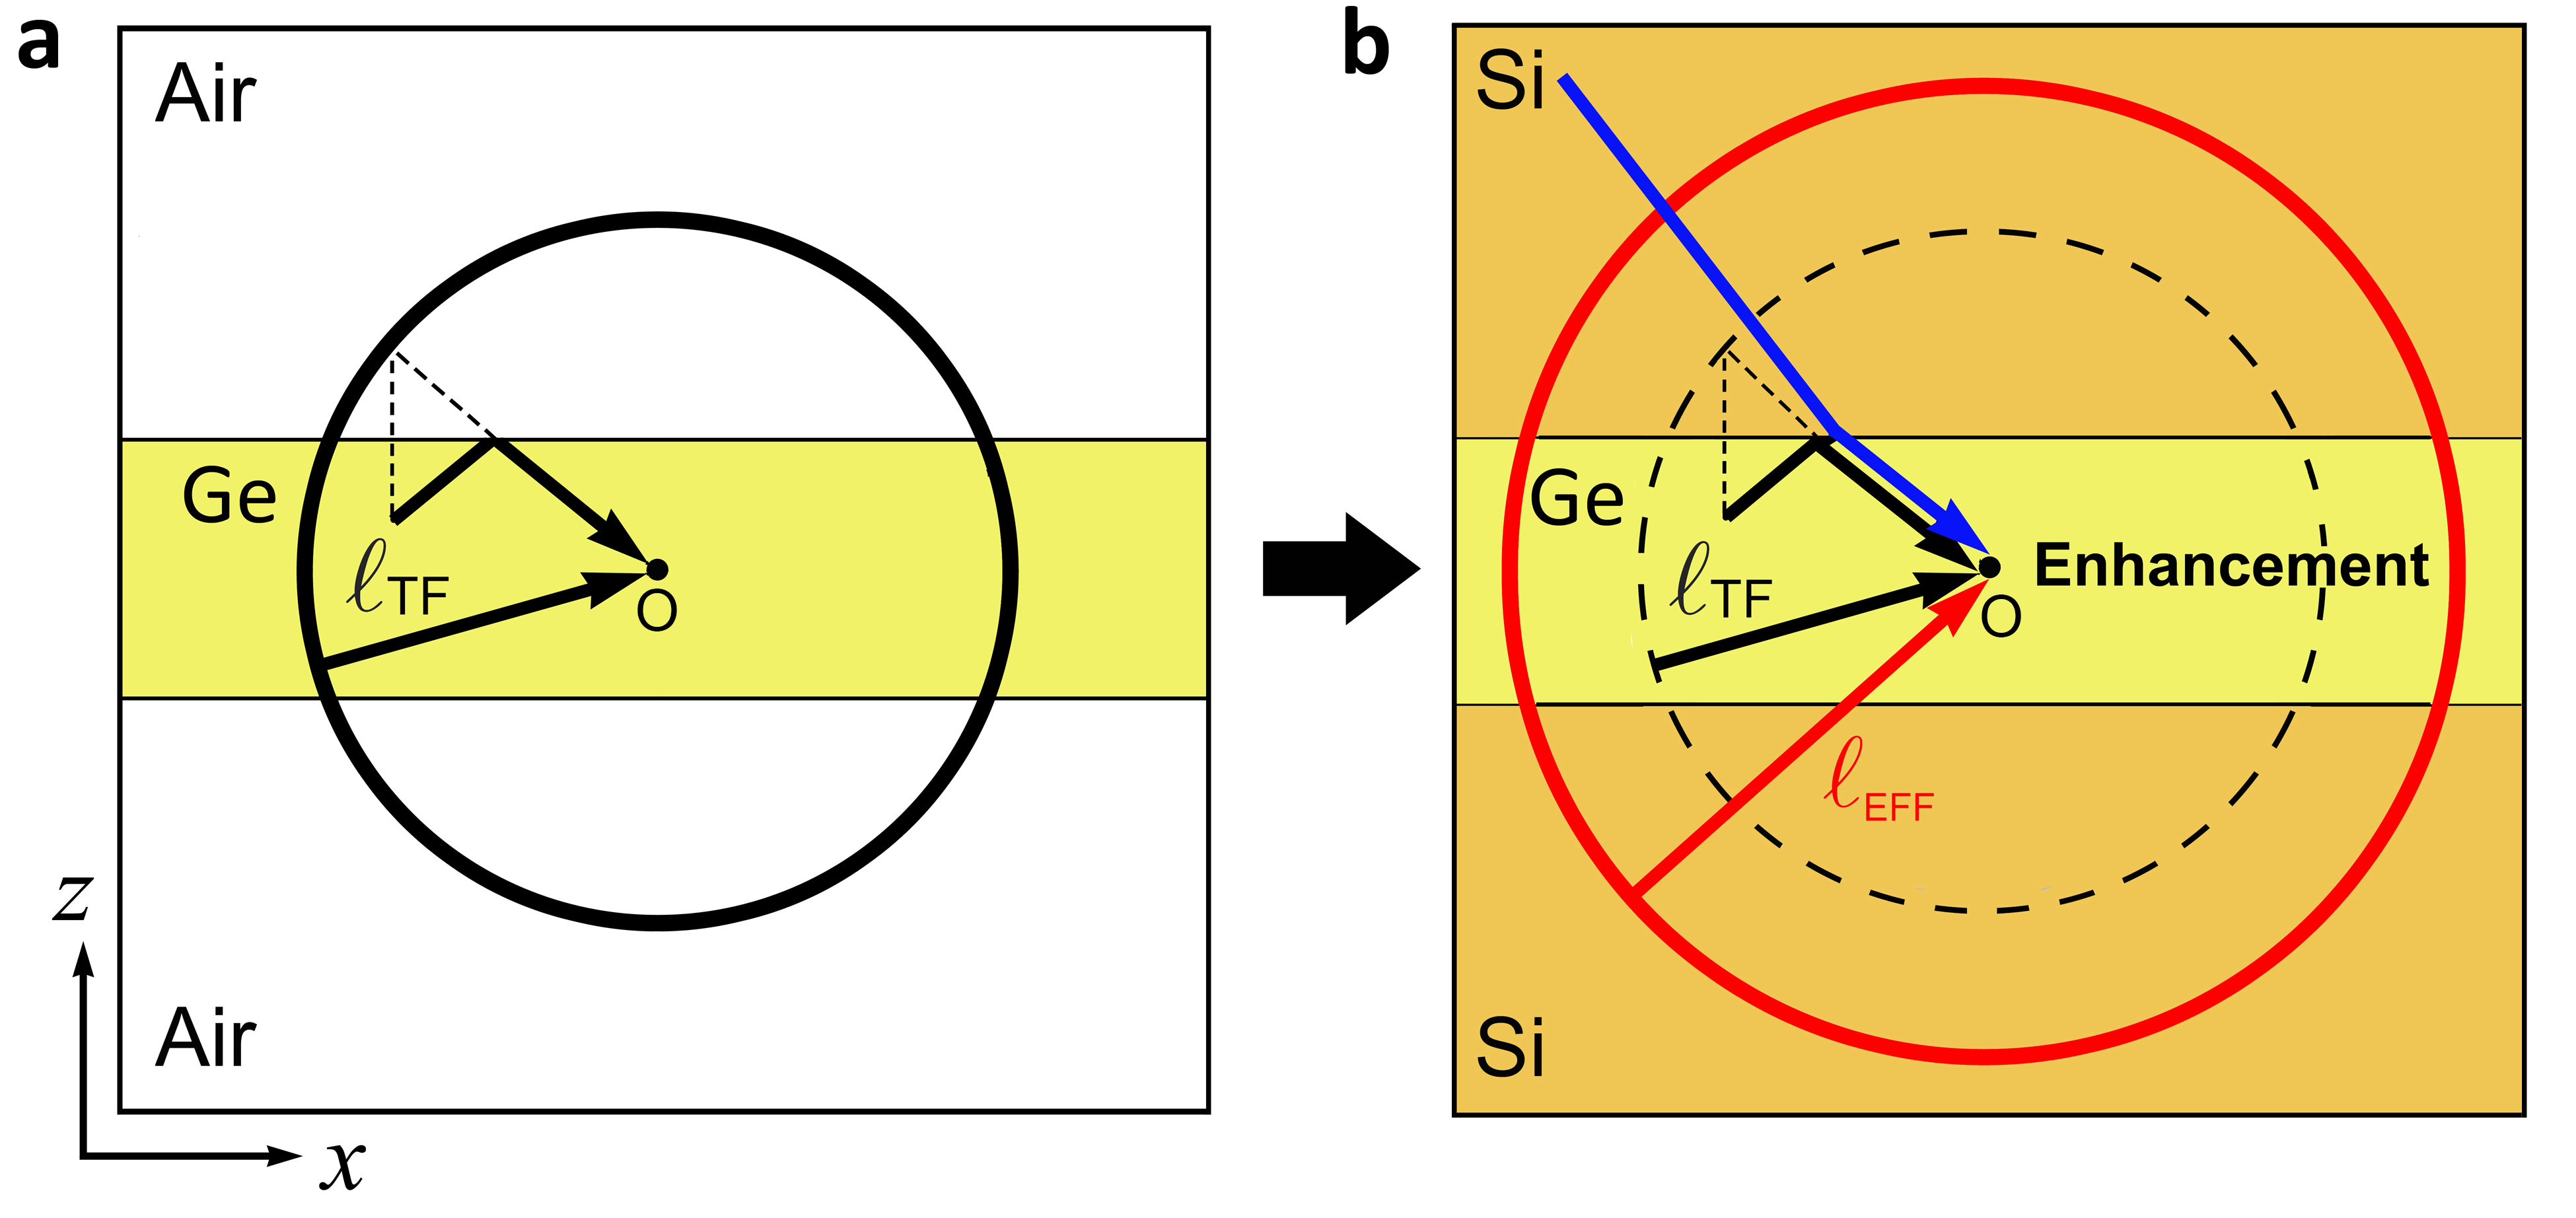
\includegraphics[width=0.90\textwidth]{figures/ch5/Fig3-enh.jpg}
  \caption{Phonon Injection. (a) Schematic for phonon contributions to the thermal conductivity of a germanium thin film under a temperature gradient along the $x$-direction. The thermal flux at point O is carried by phonons whose last collision was, on the average, at a distance of mean free path $\ell_{\text{TF}}$ away from O, as represented by the black circular line. For simplicity we neglect the angular dependence of $\ell_{\text{TF}}$. (b) When the germanium film is in contact with the silicon film, phonons from silicon can be injected into germanium (blue). These phonons had their last collision at a larger distance than those arriving from germanium. As a result, the effective mean free path $\ell_{\text{EFF}}$ is larger (red) and the thermal conductivity at point O is enhanced.}
    \label{fig:ch5-enh3}
\end{figure}
\par To further explain the origin of the thermal conductivity enhancement, we analyze the transport behavior of a well-established system of a “nanoparticle-in-alloy” bulk semiconductor \cite{RN98,RN29} and compare it with our nanostructured semiconductor. In a bulk structure, the thermal conductivity at a point O in real space is determined on an average by phonons coming from a spherical surface centered at that point with radius equaling the bulk mean free path in that semiconductor. Any changes to the semiconductor structure (such as addition of alloy atoms and nanoparticles) outside this “influence-sphere” can be considered to minimally affect the thermal conductivity at the point O. On the other hand, the inclusion of alloy atoms and nanoparticles within this influence-sphere will reduce the thermal conductivity by shortening the bulk phonon mean free paths, thereby reducing the effective radius of the influence-sphere. Analogous to the bulk case, in the case of a free standing thin-film [\Cref{fig:ch5-enh3}(a)], the thermal conductivity at a point O inside the film is determined on an average by phonons arriving from the surface of the influence sphere (see black circular line) given by the thin-film mean free path. We analyze the phonon trajectories and the impact of scattering on the effective phonon mean free paths for the germanium thin film and the tri-layer superlattice structure in \Cref{fig:ch5-enh3}. The addition of the silicon cladding layers to the germanium thin film [\Cref{fig:ch5-enh3}(b)] ensures that in addition to the phonons within the germanium layer, transmitted phonons from silicon that can couple across the interface and reach point O are able to enhance the thermal conductivity by increasing the effective mean free paths (red circle). This is because phonons arriving from silicon through transmission had their last collision on an average at a larger distance than those arriving from germanium. Consequently, we show that nanostructuring does not necessarily lead to a reduction in the germanium thermal conductivity, alternatively it can generate an enhancement of heat conduction.
\subsection{Reduction in Si Layer Conductivity} 
It is important to note that the increase of $\kappa_{\text{Ge}}$ should not be interpreted as an increase in the average thermal conductivity of the structure due to the addition of material (Si) with higher conductivity. In fact, here we show that the Si cladding layers reduce their thermal conductivities in the Si-Ge-Si tri-layer structure. We calculate the thermal conductivity $\kappa_{\text{Si}}$ of the outer cladding layers of Si in \Cref{fig:ch5-red1}. 
%Figure
\begin{sidewaysfigure}[hbtp]
  \centering 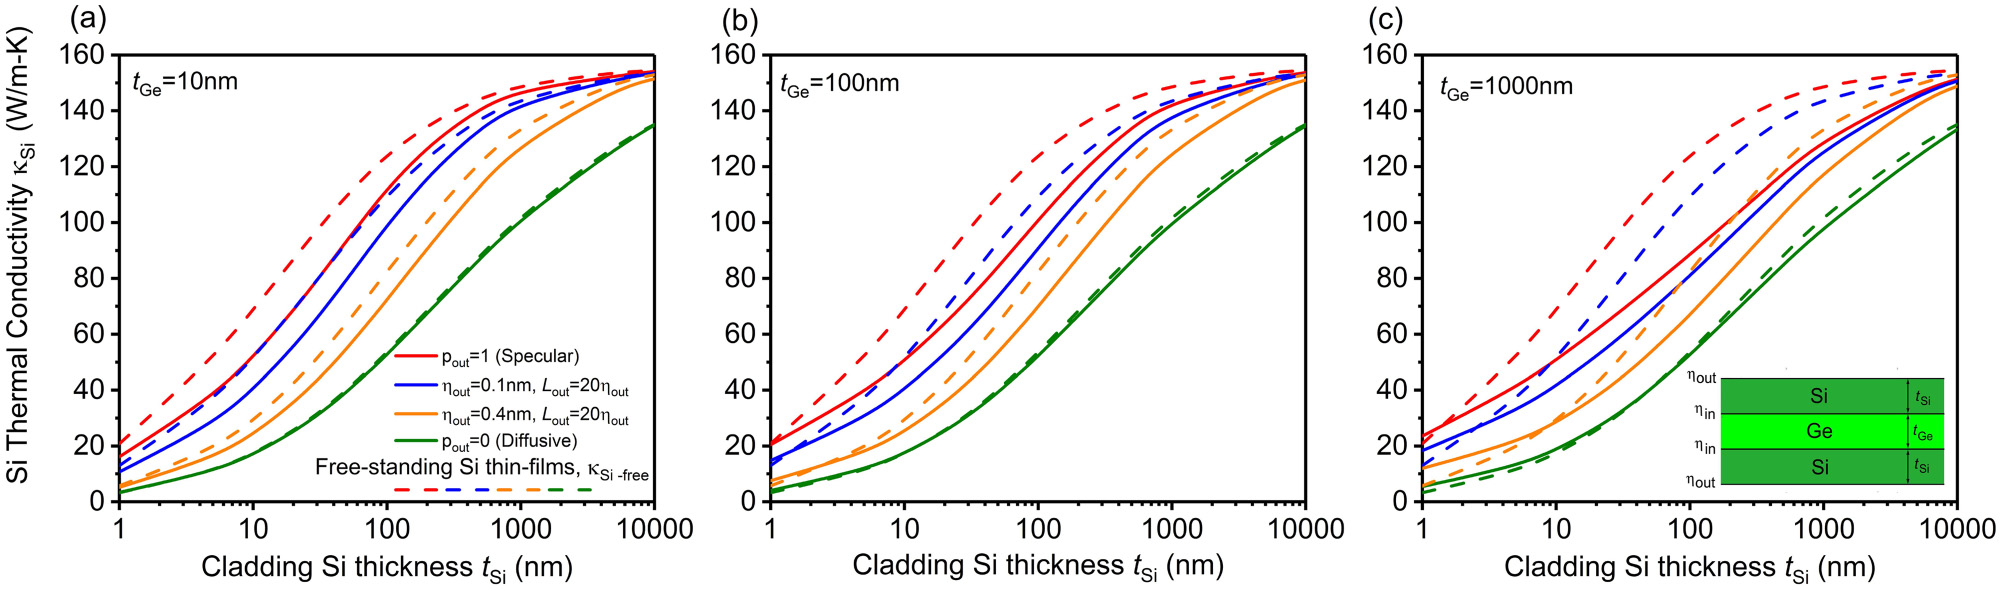
\includegraphics[width=1.0\textwidth]{figures/ch5/Fig1-red.jpg}
  \caption{Thermal conductivity of a cladding Si layer in a Si-Ge-Si architecture for different embedded layer thicknesses $t_{\text{Ge}}$ of (a) 10 nm, (b) 100 nm, and (c) 1000 nm. The inner roughness $\eta_{in}$ is 0.1 nm. The plots show the dependence of the thermal conductivity $\kappa_{\text{Si}}$ on cladding layer thickness $t_{\text{Si}}$ and outer Si-air interface conditions. The corresponding Si free-standing thin-film conductivity $\kappa_{\text{Si-free}}$ is shown for reference with dotted lines.}
    \label{fig:ch5-red1}
\end{sidewaysfigure}
In this system, the outer interface is defined as the interface between the outer Si layer and air and the inner interface is between Ge and Si layers. Note that the surface conditions of the baseline free-standing Si film are the same as the cladding Si layer in the tri-layer structure, i.e., roughness of the Ge-Si interface on one side and the roughness of the Si-air interface on the other, in order to obtain a comparison with same surface conditions and independently study the effects of phonon coupling between layers. In general, we find that $\kappa_{\text{Si}}$ falls below its corresponding free-standing thin-film value $\kappa_{\text{Si-free}}$. This result shows that the Si layer acts as a “net injector” of phonons into the Ge layer thereby reducing its own conductivity. We find that the reduction in $\kappa_{\text{Si}}$ in comparison to $\kappa_{\text{Si-free}}$ is larger for (a) thick Ge embedded layers and (b) smooth outer surfaces. A larger reduction in $\kappa_{\text{Si}}$ from $\kappa_{\text{Si-free}}$ for larger $t_{\text{Ge}}$ is obtained since more injected phonons travel in the Ge layer reducing the mean-free-paths below the freestanding values. For small $t_{\text{Ge}}$, phonons from one Si layer can travel across the Ge layer into the other Si layer (which possesses higher transport properties) thereby reducing their thermal conductivity to a lesser degree. In the case of a fully diffusive outer surface, the reduction of $\kappa_{\text{Si}}$ from $\kappa_{\text{Si-free}}$ is small since those phonons in the Si layer that interact with the diffusive interface are prevented from being reflected and thus being injected into the Ge layer. Thus, a strong shortening of phonon mean-free-paths in the Si layer effectively reduces the injection of phonons into the embedded layer. We note that the increase in $\kappa_{\text{Si}}$ with increasing thickness $t_{\text{Si}}$ is a consequence of the reduction of phonon surface scattering in the quasi-ballistic regime and not due to phonon coupling effects and is thus observed for both free-standing Si thin-films (dashed lines) and Si-layer in the tri-layer architecture (solid lines). To understand the role played by inner interface properties, we increase the inner Ge-Si roughness to $\eta_{in}$ = 0.4 nm as shown in [\Cref{fig:ch5-red2}]. The increased $\eta_{in}$ lowers the coupling of phonons between cladding and embedded layers as more phonons get diffusively scattered at the rougher interface (\Cref{eq:bezak_transmission}). The reduced phonon coupling for $\eta_{in}$ = 0.4 nm is manifested as a lesser reduction of $\kappa_{\text{Si}}$ with respect to $\kappa_{\text{Si-free}}$ [\Cref{fig:ch5-red2}] in comparison to $\eta_{in}$ = 0.1 nm [\Cref{fig:ch5-red1}]. For very large surface roughnesses $\eta_{in}$ (e.g., $p_{in}$ = 0), all the layers can be treated as decoupled from each other and, in that case, all phonon coupling effects on thermal transport would be negligible. 
%Figure
\begin{sidewaysfigure}[hbtp]
  \centering 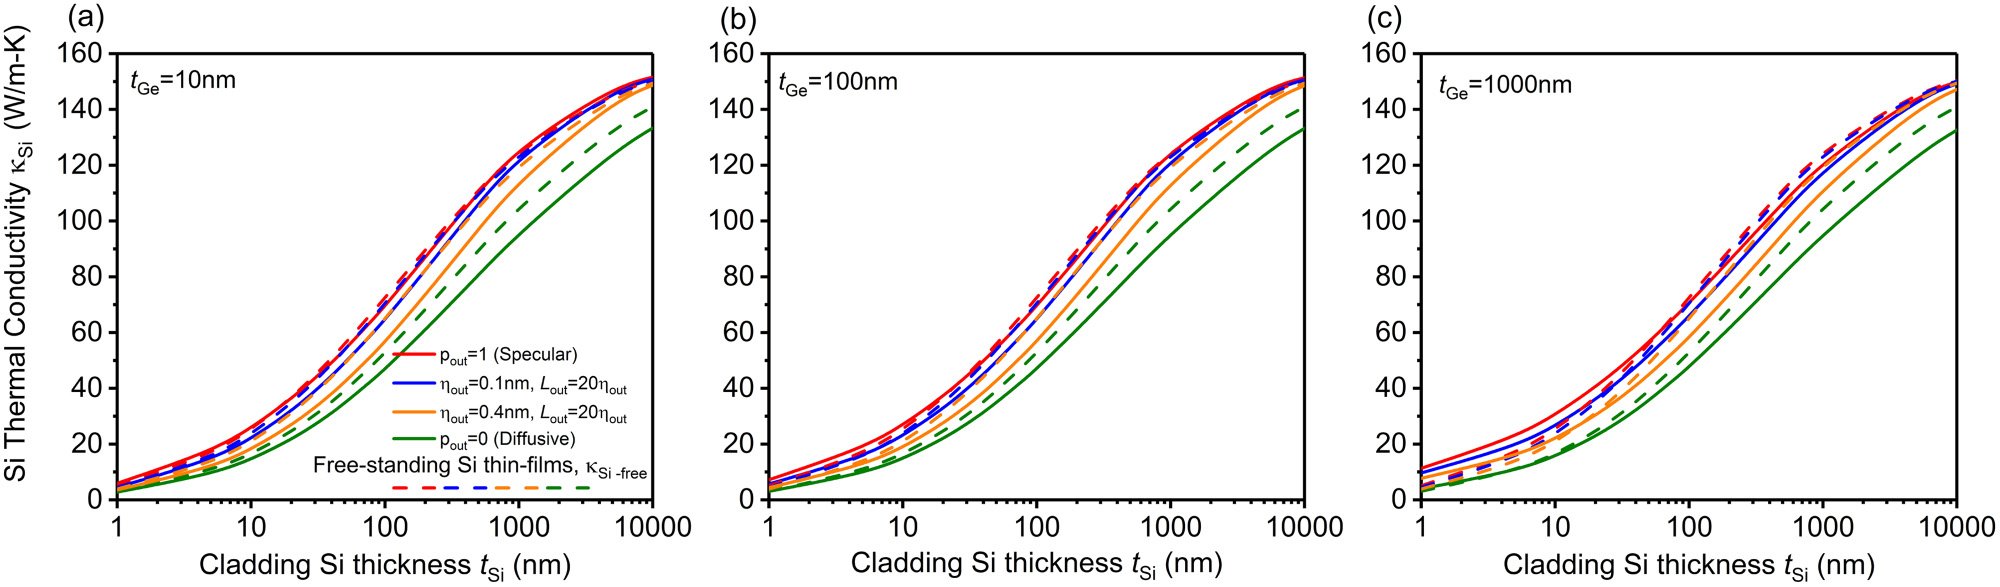
\includegraphics[width=1.0\textwidth]{figures/ch5/Fig2-red.jpg}
  \caption{Thermal conductivity of embedded Si layer $\kappa_{\text{Si}}$ in a Si-Ge-Si architecture with inner roughness $\eta_{in}$ = 0.4 nm as a function of cladding layer thickness $t_{\text{Si}}$. The thickness of the embedded layer $t_{\text{Ge}}$ is increased from (a) 10 nm, (b) 100 nm to (c) 1 \si{\micro}m, and four outer surface conditions are considered -- specular, $\eta_{out}$ = 0.1 nm, $\eta_{out}$ = 0.4 nm, and diffuse.}
    \label{fig:ch5-red2}
\end{sidewaysfigure}

\subsection{Si-Ge Bi-layers}
 We have focused our previous analysis on tri-layer structures made of Si and Ge with varying layer spacing to analyze the coupling of phonons between the layers and understand the impact on thermal conductivity modulations in each layer. Since the mechanism of phonon coupling is independent of the number of layers, the analysis can be extended to any arbitrary $n$-layered structure. We note that structures with $n$ = 2, i.e., bi-layers are a common experimentally grown structure, and the experimental measurement of each layer’s thermal conductivity \cite{RN189,RN126} could potentially be easier to achieve as compared to a tri-layer system. With the motivation for guiding future experiments, we briefly analyze the thermal conductivity modulations in a bi-layer system of Si and Ge with thickness of each layer given as $t_{\text{Si}}$ and $t_{\text{Ge}}$. We note that for a Si-Ge bi-layer, the system of equations to evaluate deviation functions \gls{g}$_i$ for layer-1 (Si) and layer-2 (Ge) can be easily extended to account for the changed boundary conditions from the tri-layer system discussed earlier. In a Si-Ge bi-layer system, three interfaces exist--the top Si-air interface, the Si-Ge interface, and the bottom Ge-air interface. For simplicity, we assume identical interfacial conditions for both the outer Si-air and Ge-air interfaces. Thermal conductivity modulations in three structures with different thicknesses of silicon and germanium (i) $t_{\text{Si}}$= $t_{\text{Ge}}$ = 10 nm, (ii) $t_{\text{Si}}$ = 100 nm, $t_{\text{Ge}}$ = 10 nm, and (iii) $t_{\text{Si}}$= $t_{\text{Ge}}$ = 100 nm are considered to elucidate the impact of phonon coupling. \Cref{fig:ch5-bilayer} shows that analogous to tri-layer structures, silicon thermal conductivity $\kappa_{\text{Si}}$ is reduced below its free standing thin-film value $\kappa_{\text{Si}}$-free when phonons originating in Si are injected into Ge causing a corresponding enhancement in $\kappa_{\text{Ge}}$. The impact of phonon coupling on thermal conductivity modulations in each layer is stronger when the inner surface is smoother as indicated by the larger differences in layer thermal conductivities in top panels in contrast to bottom-panels of \Cref{fig:ch5-bilayer} from their respective free-standing values. The enhancement in $\kappa_{\text{Ge}}$ is higher when silicon layer thickness $t_{\text{Si}}$ is large, while the reduction in $\kappa_{\text{Si}}$ is higher when germanium layer thickness $t_{\text{Ge}}$ is larger, clearly indicating the reciprocity in phonon injection process as was observed in tri-layer architectures. These findings would be useful for future experimental investigations into phonon coupling.
 %Figure
\begin{figure}[hbt]
  \centering 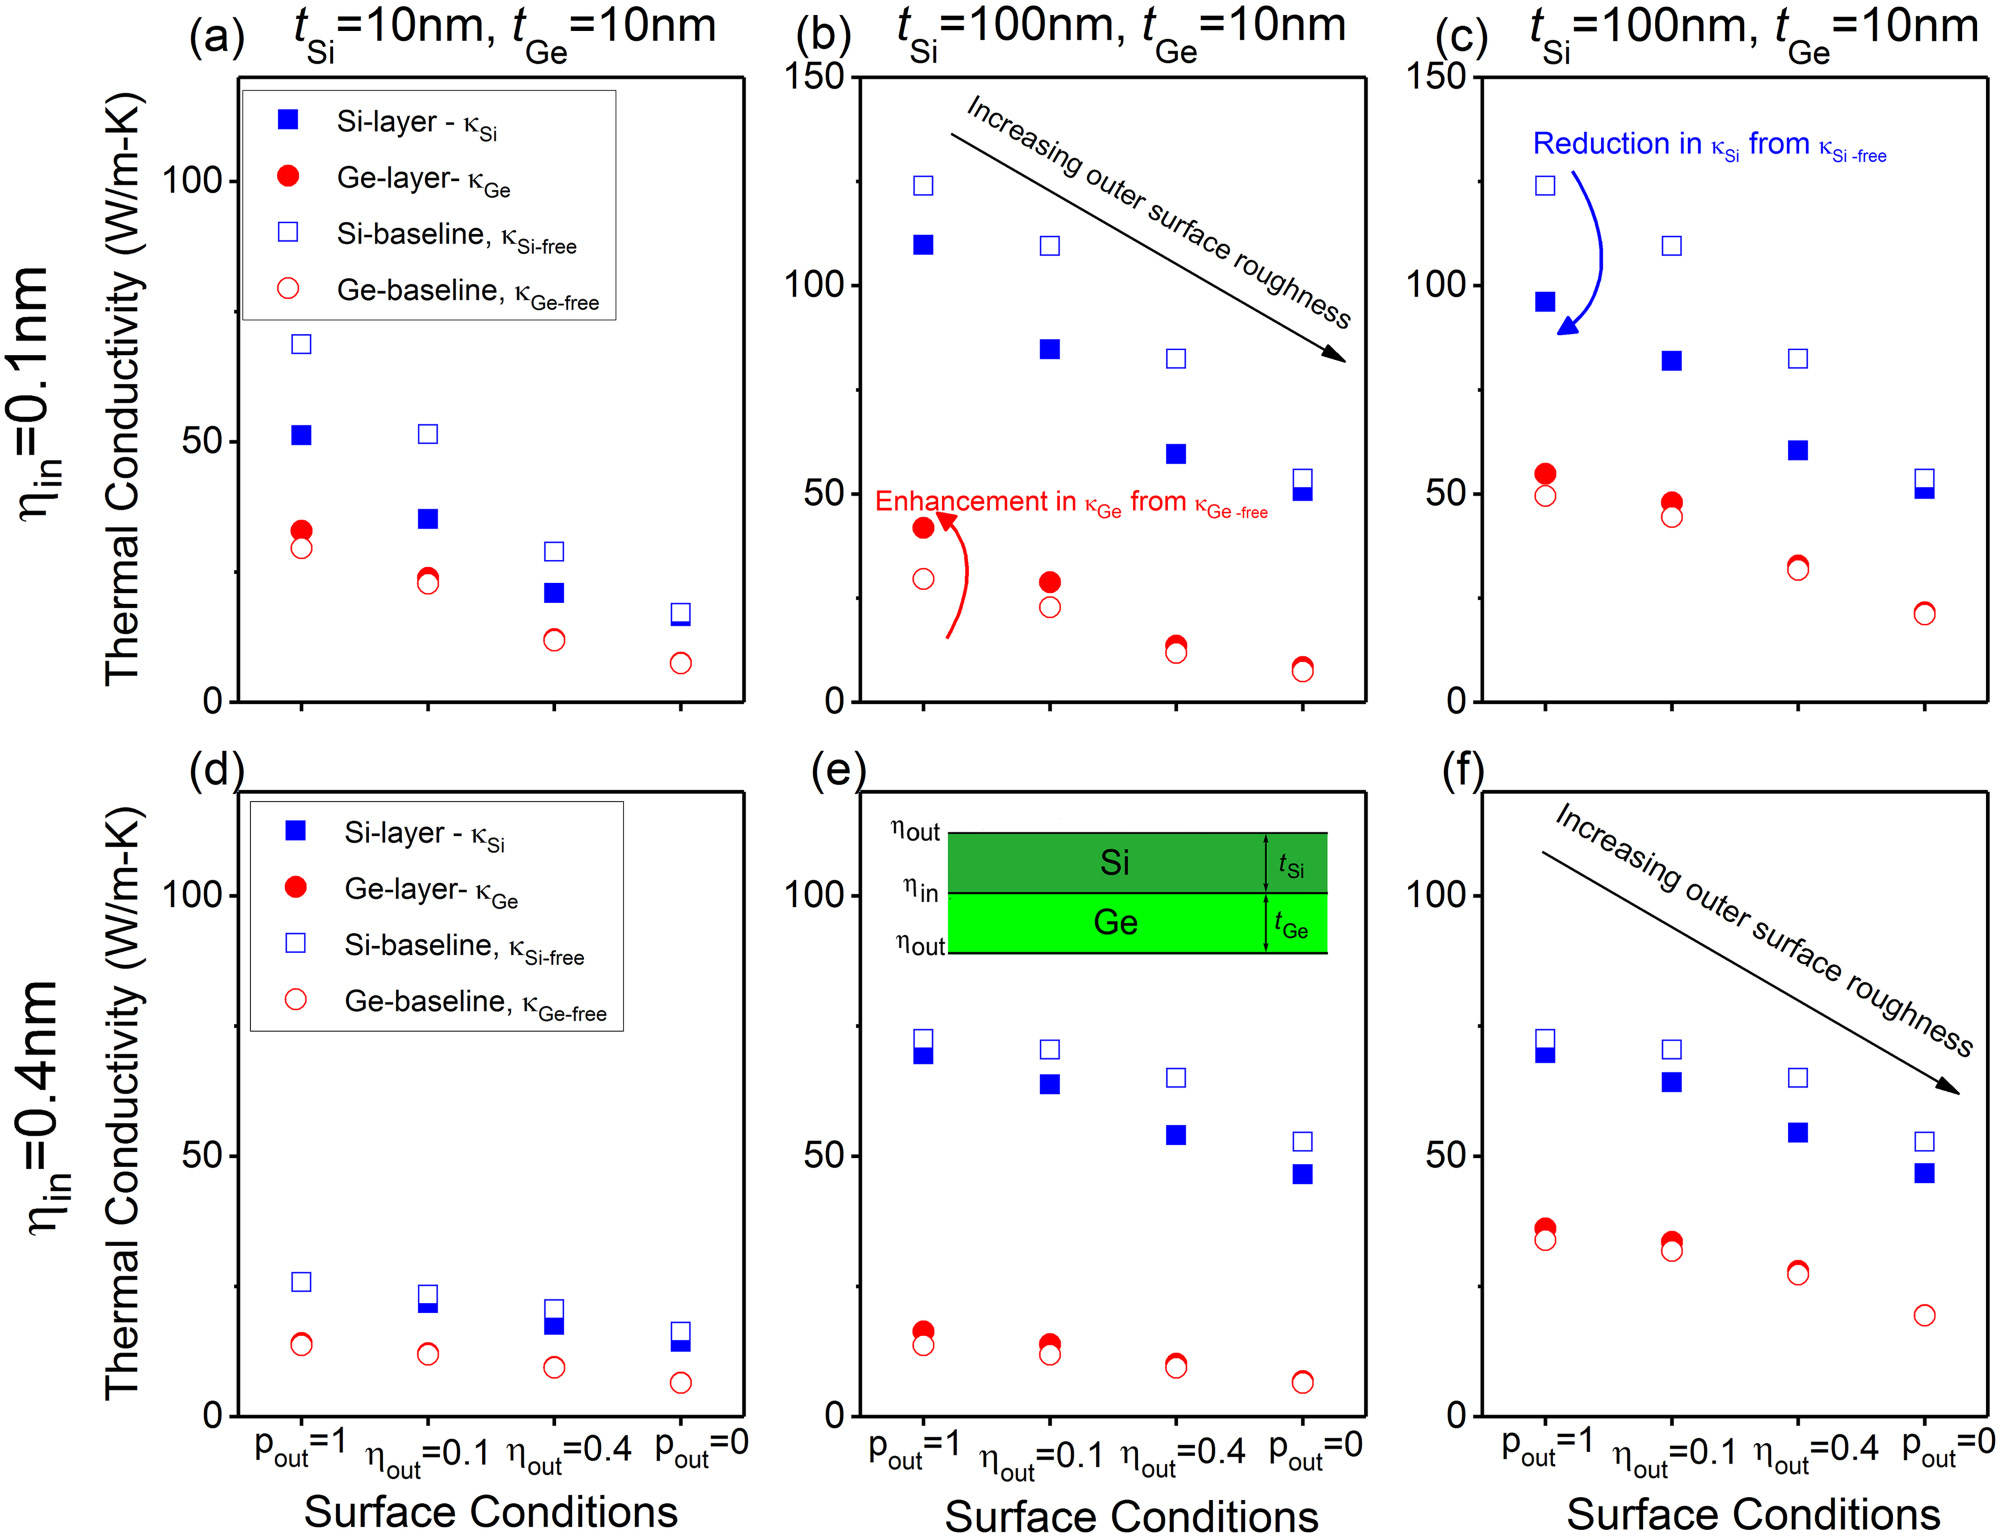
\includegraphics[width=1.0\textwidth]{figures/ch5/Fig4.jpg}
  \caption{Thermal conductivity of layers of silicon $\kappa_{\text{Si}}$ (solid blue square) and germanium $\kappa_{\text{Ge}}$ (solid red circle) in bi-layer structures with different silicon and germanium layer thicknesses: [(a), (d)] $t_{\text{Si}}$= $t_{\text{Ge}}$= 10 nm, [(b), (e)] $t_{\text{Si}}$= 100 nm, $t_{\text{Ge}}$ = 10 nm, and [(c), (f)] $t_{\text{Si}}$ = $t_{\text{Ge}}$ = 100 nm. Top panels correspond to inner roughness $\eta_{in}$ = 0.1 nm and bottom panels to $\eta_{in}$ = 0.4 nm. Four different outer surface conditions are shown on the $x$-axis in each panel -- specular, $\eta_{\text{Si-air}}$ = $\eta_{\text{Ge-air}}$  = 0.1 nm, $\eta_{\text{Si-air}}$ = $\eta_{\text{Ge-air}}$ = 0.4 nm, and diffuse. Open symbols represent the corresponding free-standing thin-film conductivity $\kappa_{\text{Si-free}}$ (blue) and $\kappa_{\text{Ge-free}}$ (red).}
    \label{fig:ch5-bilayer}
 \end{figure}
 %
\subsection{Films-on-substrate}
We also consider a baseline physical system consisting of a thin-film of material A on top of a substrate of material B. Our choice of A and B is motivated from optoelectronic applications such as photo-detectors where configurations based on Si, Ge, GaAs and AlGaAs semiconductors are found ubiquitously \cite{book_rogalski_infrared,RN387,ownKK1}. We focus on studying the influence of this semi-infinite substrate on the thermal conductivity modulation in the film-on-substrate (FOS) system [\Cref{fig:ch5-fos1}] and contrast the unique behavior with free-standing isolated thin films.
%Figure
\begin{figure}[hbt]
  \centering 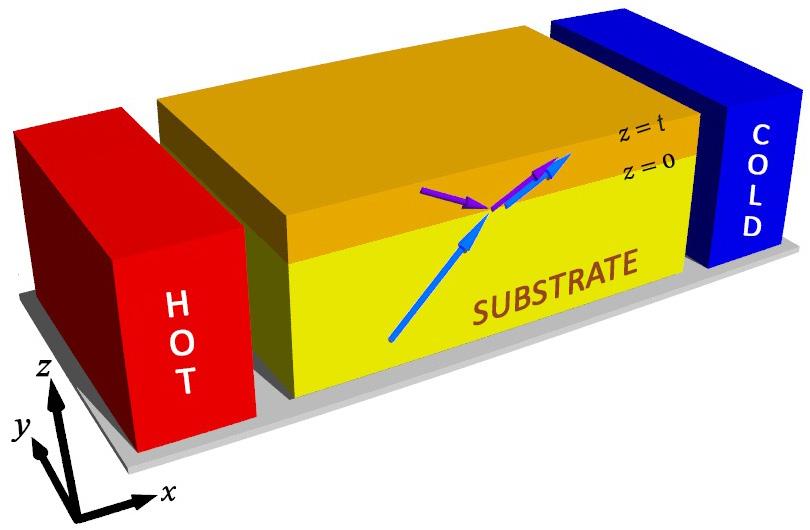
\includegraphics[width=0.75\textwidth]{figures/ch5/Fig5-fos1.jpg}
  \caption{Schematic of a film-on-substrate (FOS) architecture where the film is shown in orange and the substrate in yellow. Arrows represent phonons originating at the film and the substrate and contributing to film phonon transport after reflection and transmission (inter-layer coupling).}
    \label{fig:ch5-fos1}
 \end{figure}
 %Figure
\begin{figure}[hbt]
  \centering 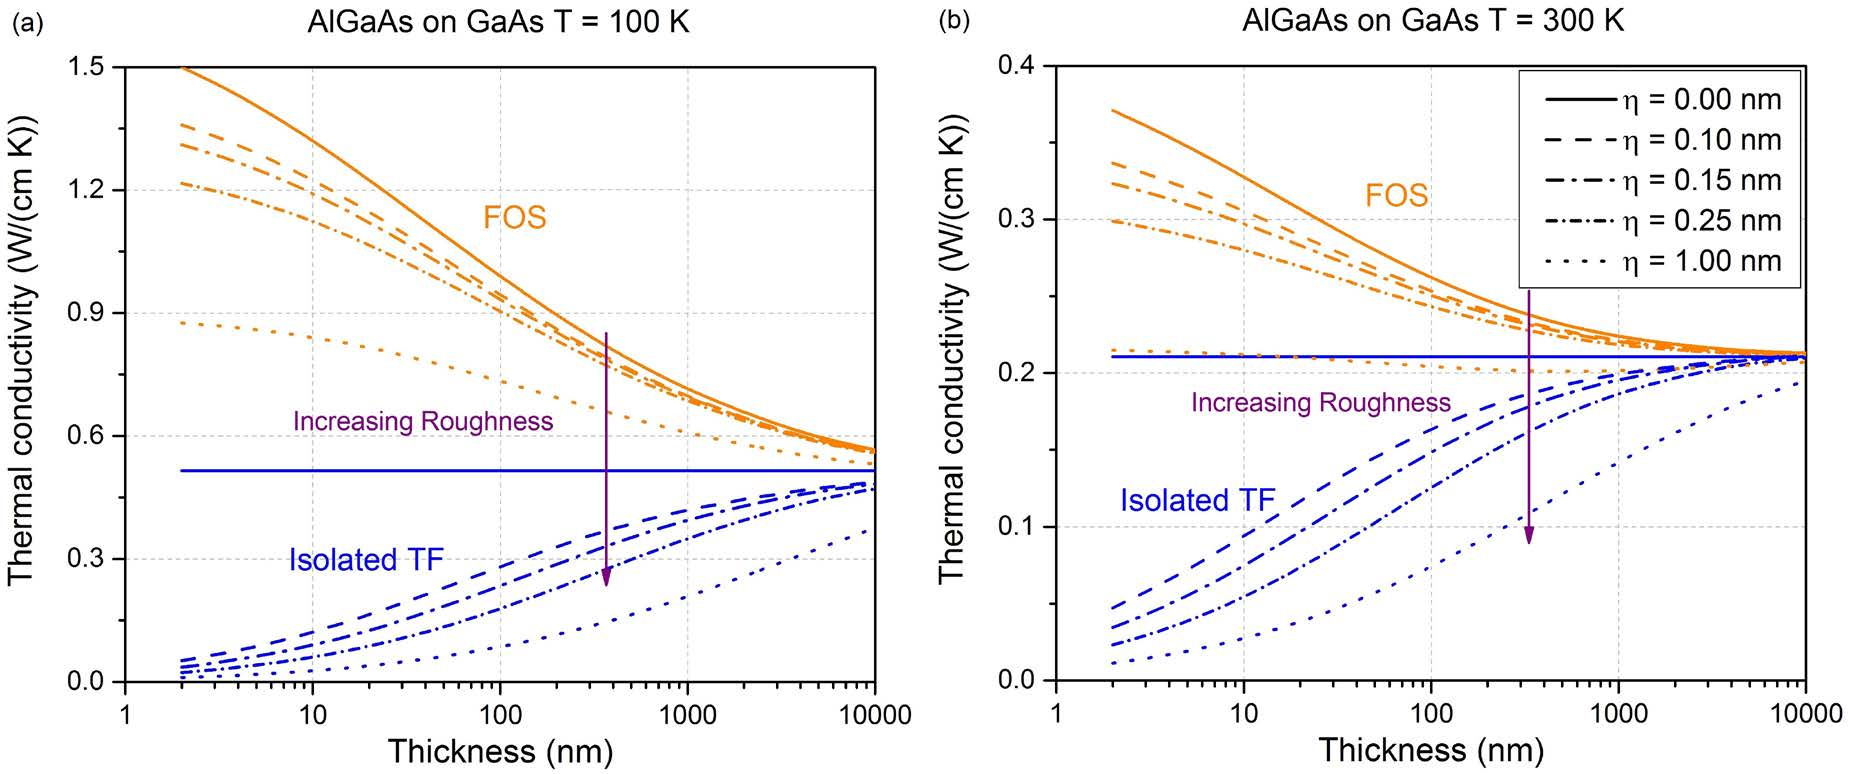
\includegraphics[width=1.0\textwidth]{figures/ch5/Fig5-fos2.jpg}
  \caption{Thermal conductivity of an \algas{0.10}{0.90} thin film grown on GaAs substrate in FOS architecture (orange lines) and an isolated free-standing \algas{0.10}{0.90} thin film (blue lines) for different interfacial roughnesses at temperatures (a) \gls{T} = 100 K and (b) \gls{T} = 300 K. The vertical arrow denotes the direction of increasing roughness. Blue horizontal line corresponds to the bulk thermal conductivity of \algas{0.10}{0.90}.}
    \label{fig:ch5-fos2}
 \end{figure}
 \par We show in \Cref{fig:ch5-fos2} the predicted thermal conduction variation of a ternary alloy \algas{0.10}{0.90} thin film atop a GaAs substrate for the case of equal inner and outer surface conditions, while varying the thickness of the \algas{0.10}{0.90} thin film. Our calculations show that the thermal conductivity $\kappa$ of the thin film in the FOS architecture increases with decreasing thickness, which is exactly the opposite of the conventional free-standing calculations \cite{RN204,ownTF} which predict that it decreases. Specifically, we found that the thermal conductivity of a thin-film in a FOS structure can be larger than the bulk thermal conductivity (horizontal blue line) as well as that of an isolated, free-standing film of the same material with similar structural properties. The observed enhancement in the thermal conductivity ($\Delta\kappa$) of the \algas{0.10}{0.90} film is attributed to phonon injection from the substrate \cite{ownCoupling1}. For certain surface conditions, interfacial coupling between the thin film and the substrate allow phonons to be exchanged between the two media. In the FOS case, the phonon mean-free-paths of the substrate material are larger than their corresponding thin-film phonon mean-free-path. Since the local thermal conductivity at a point inside the thin film is determined by the effective mean-free-path of phonons reaching that point, the local thermal conductivity of the thin-film in the FOS structure is enhanced beyond the isolated thin-film value due to an injection of larger mean-free-path phonons from the substrate, which leads to a larger effective mean-free-path for phonons in the thin-film. For the case when phonons in the thin film have larger mean-free-paths compared to the substrate, the thermal conductivity of the FOS would be smaller than the corresponding isolated thin-film. It is noteworthy that the thermal conductivity $\kappa$ of the film can be enhanced beyond the \algas{0.10}{0.90} bulk conductivity value. We denote this enhancement of thermal conduction beyond the bulk conductivity values by $\Delta\kappa_{\text{bulk}}$ whereas we denote the enhancement beyond isolated thin film conductivity values as $\Delta\kappa_{\text{iso}}$. We remark that we observe an increasing $\Delta\kappa_{\text{bulk}}$ with reducing thickness of thin film for a wide range of interfacial roughnesses. This finding can have profound consequences since achieving enhanced thermal conduction is a key component of enabling heat dissipation from hot spots in optoelectronic and microelectronic applications. The facilitation of effective heat dissipation in nanostructures can further promote miniaturization and efficient power consumption in devices. We observe this trend of enhancement beyond bulk conductivity $\Delta\kappa_{\text{bulk}}$ to be significant even at \gls{T} = 300 K, which shows that devices will be competent for room temperature operation as well. We note that, the unconventional increase in the thermal conductivity of the thin film in the FOS architecture with decreasing thickness can be understood in light of recognizing the role of interfacial scattering and film thickness. For small roughnesses, we have low diffusive interfacial scattering, and due to the low acoustic impedance mismatch between \algas{0.10}{0.90} and GaAs there is a strong inter-layer phonon coupling in the system. With decreasing film thickness, the volume fraction in the film in which there is an enhancement of thermal conductivity arising from inter-layer phonon coupling increases because phonons being injected from GaAs, which have finite mean-free-path, are allowed to influence a larger film proportion. As a result, the thermal conductivity $\kappa$ of the film increases with decreasing thickness for $\eta$ = 0, 0.10, 0.15 and 0.25 nm because the enhancement by phonon coupling is larger than the decrease by diffuse interface scattering. On the other hand, for the isolated free-standing thin film, we observe a reduction in thermal conductivity with decreasing thickness, which is due to conventional boundary scattering. Note that in this case there is no inter-layer phonon coupling and therefore there are no physical mechanisms to observe an increase in heat conduction. Significantly, we found that the different physical mechanisms behind thermal transport in isolated and FOS films can lead to opposite thermal conductivity behaviors when the film thickness is reduced. We note that we investigate the thermal conductivity of the thin film atop the substrate and not that of the entire structure consisting of the substrate and thin film. \Cref{fig:ch5-fos2} also shows how the thermal conductivity increases with reducing roughness and temperature. We remark that for case of very rough interfaces (e.g. $\eta$ = 1.0 nm) and \gls{T} = 300 K [\Cref{fig:ch5-fos2}(b)], we observe a minimum in thermal conductivity for a film thickness close to \gls{t} = 500 nm, which is due to the competition between thermal conductivity enhancement by phonon coupling and thermal conduction reduction by interfacial scattering. We highlight that this minimum in thermal conductivity is independent of any thermal phonon wave effects or coherent heat conduction which have been reported in other studies \cite{RN253,RN393}. 
 %Figure
\begin{figure}[hbt]
  \centering 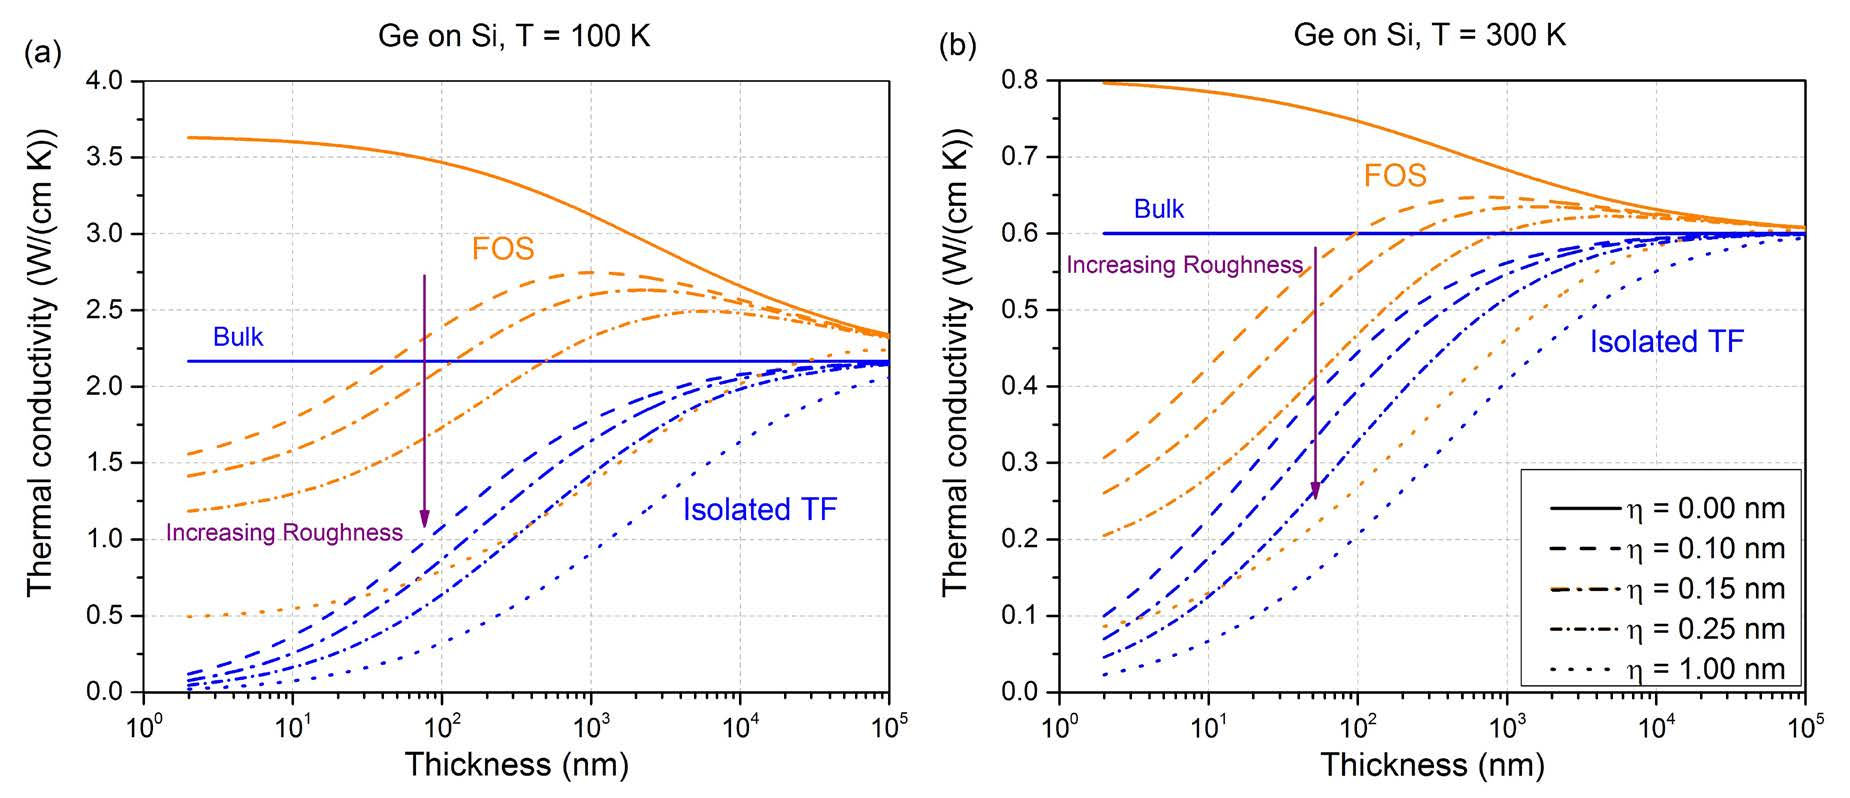
\includegraphics[width=1.0\textwidth]{figures/ch5/Fig5-fos3.jpg}
  \caption{Thermal conductivity of a Ge thin film grown on Si substrate in FOS architecture and an isolated free-standing Ge thin film depicted by orange and blue lines respectively for different interfacial roughnesses at temperatures (a) \gls{T} = 100 K and (b) \gls{T} = 300 K. Blue horizontal line corresponds to bulk thermal conductivity of Ge.}
    \label{fig:ch5-fos3}
 \end{figure}
\par In \Cref{fig:ch5-fos3}, we consider an FOS system consisting of a thin film of Ge deposited on a Si substrate, where we study the variation of thermal conductivity of the FOS film and contrast it with that of bulk Ge and an isolated thin film of Ge. Our numerical predictions show that for certain surface conditions and thicknesses the thermal conductivity of the thin film on substrate still increases beyond the bulk Ge thermal conductivity with decreasing thickness but enhancement effects by phonon coupling are less pronounced in this case due to dissimilar dispersion relations for Si and Ge. The thermal conductivity of FOS is also enhanced beyond the corresponding isolated thin film conductivity values. We note that a large acoustic impedance between Si and Ge owing to a difference in densities and phonon mode velocities leads to significant reduction in transmission and phonon coupling in the Si-Ge case. Thus, with decreasing thickness, we generally observe a decrease in the thermal conductivity of the FOS due to increasing diffuse scattering effects. However, for cases where the interfacial diffuse scattering is not the dominant mechanism (for instance, when $\eta$ = 0) the thermal conduction increases since the volume fraction in which the enhancement takes place increases with decreasing spacing. These combined mechanisms for phonon transport (phonon coupling and interface scattering) also explain the maxima observed in the thermal conductivity of the FOS Si-Ge system. We also mark that the thermal conductivity enhancement ($\Delta\kappa_{\text{iso}}$), diminishes with increasing thickness of the thin film. This is due to the reducing influence of surface scattering and phonon coupling and the fact that thin film conductivities tend towards the bulk conductivity with increasing thickness. We also show in \Cref{fig:ch5-fos3} the impact of surface conditions and temperature variation and find how the thermal conductivity and its enhancement increases with reduction in surfaces roughness and temperature.
\par In contrast to established thermal transport in thin-films, we showed that it is possible to increase the in-plane thermal conductivity of a thin film by placing it on top of an appropriate substrate and that the thermal conductivity increases with decreasing spacing. We observe enhancement of thermal conductivity in FOS architecture beyond the predictions for bulk and isolated thin-film and study its behavior with changing thickness, roughness and temperature. AlGaAs on GaAs and Ge on Si, as considered in this chapter, are widely used as fundamental units in electronic and optoelectronic applications. The analysis of these FOS architectures suggests that experimental measurement of thermal conductivity of thin-films needs to account for thermal coupling between thin film and substrate and the consequent conductivity modification and indicates the need to develop rigorous conductivity read-out model for experiments. 
\section{Summary}
In this chapter, we presented a novel approach of phonon spectral coupling to modulate the thermal conductivities of nanomaterials. We first analyzed the underlying reasons behind thermal conductivity reduction of cladding Si layers in a Si-Ge-Si architecture with simultaneous thermal conductivity enhancement of embedded Ge layer. We also investigated the thermal conductivity of each layer in a Si-Ge bi-layer architecture which was extended to the experimentally important case of film-on-substrate systems. The overall phenomena underlying these modifications were discovered to be phonon injection due to spectral coupling across the interfaces in these materials. The complex nature of this injection mechanism manifests itself in unique and novel modifications to thermal conductivities. The enhancement and reduction in thermal conductivities depends on both structural and materials properties. The findings in this study are a critical step toward achieving a comprehensive control over the thermal properties of materials. By providing capabilities to enhance thermal conductivities, technologies such as microelectronics can be made more efficient by achieving high thermal dissipation rates. At the same time, reducing thermal conduction by combining phonon spectral coupling and current diffuse scattering approaches can improve the performance of thermoelectrics. The proposed phonon spectral coupling to modulate heat conduction advances the current understanding of phonon transport in nanostructures, creating new opportunities for thermal materials design and development.

